\documentclass{article}

\usepackage{hyperref}
\usepackage{graphicx}
\usepackage{amsmath}
\usepackage{float}



\hypersetup{
    colorlinks = true,
    linkcolor = blue,
    anchorcolor = blue
}

\graphicspath{{img/}}





\title{Heat Dissipation}

\author{Davide Dal Bianco \\ 2598719}

\begin{document}

\maketitle

\section{Introduction} \label{sec:introduction}
In this report we will introduce the implementation and the parallelization of a program which simulate the heat dissipation on a cylindrical surface. In order to simulate the dissipation, the time domain is discretized and the procedure iterates until it converges or the maximum number of iterations is reached. The program will be implemented in Cray Chapel, a modern programming language that allows to develop parallel programs using a global view programming approach, that is, the programmer solves the whole problem like a sequential program. In fact, we will provide a sequential program, a parallel (single machine) one and distributed one with minimal changes in the code. However, we will show that the compiler has many limitations and the overall performance is really bad.

\section{Algorithm} \label{sec:algorithm}
The algorithm is pretty similar to Successive Over Relaxation, except that the leftmost and the rightmost columns are virtually adjacent. On the other hand, the top and the bottom rows have fixed values. Finally, each cell is computed in a different way since it depend on a specific conductivity index and the weighted average of all neighbours. \\
If the matrix is distributed among the nodes using the block distribution, the communication required is $\mathcal{O}((M~+~N)~/~\sqrt{P})$ while the computation is $\mathcal{O}((M~\times~N)~/~P)$. It follows that the computation/communication ratio is good only when the problem size is much higher than the number of processes. When such condition is satisfied, the parallel algorithm is able to reach a nearly perfect linear speedup. \\
The row distribution should perform slightly better, since it does not require communication for copying the left-right columns and each process has to communicate with maximum two other processes.

\section{Sequential program}
Chapel's domain are a convenient high level abstraction for working with complex data structure. In order to compute the new values, we can use domains to execute operations at higher level. The following domains have been defined:
\begin{itemize}
    \item \texttt{BigD}, which represents all the cell included the ghost cells.
    \item \texttt{D}, which represents the cell to be computed.
    \item \texttt{Halo}, which represents the top-left cell and its halo.
\end{itemize}
Note that \texttt{Halo.translate(i,j)} is the domain that represents the $(i,j)$ cell and its halo. We also created the array \texttt{weights} over the domain \texttt{Halo}, where the inner cell is 0 and the other cells contain the relative weights for the average. \\
Before starting to compute the iterations, the top-bottom ghost cells (including the four corners) are copied since they have fixed values. Then each iteration does the following steps:
\begin{itemize}
    \item The left-right ghost cells are copied.
    \item Each cell $(i,j)$ is computed using the projection on \texttt{Halo.translate(i,j)} of the matrix, \texttt{weights} and the conductivity index. The result is saved in a temporary matrix.
    \item The maximum difference between the old and the new value of each cell is calculated.
    \item The new values are copied in the matrix.
\end{itemize}
Using the domain \texttt{Halo}, the algorithm can be implemented very easily. However, operations like \texttt{forall}, \texttt{reduce} and array assignments are not allowed because they introduce parallelism, hence high level operations operations must be implemented by means of a \texttt{for} iteration on the data structure.

\section{Parallel program}
In section \nameref{sec:introduction} we said the the parallel program has minimal changes compared with the sequential one. This is possible due to Chapel's data parallelism, that is, Chapel can execute operations on data structures in parallel using a thread pool. The parallelization is transparent from the programmer's perspective, but he must be aware of it because race conditions might invalid the correctness of the program. \\
The resulting parallel program is identical to the sequential one, except that operations on data structures are done using \texttt{forall} loops, the \texttt{reduce} operator and array assignments.

\section{Distributed program}
Once again, in order to distribute the program, only minimal changes to program are required. In particular, we have to tell the compiler that the data structures must be distributed among the locales. When defining the domain, it is possible to use a function that maps each index to a locale. Chapel already provides the functions for the most popular partitioning scheme and the programmer can also implement an arbitrary one, though this is not needed for this application. As described in section \nameref{sec:algorithm}, we can use the Block distribution of Chapel to split the matrix among the locales. Therefore, the only change in the program is on the definition of the domain \texttt{BigD}, which now is \texttt{dmapped Block(...)}.

\section{Performance measurement}
The running times of the program have been measured for the following problem sizes:
\begin{itemize}
    \item Size 1: M = 1000, N = 1000, E = 0.1, I = 100
    \item Size 2: M = 2000, N = 2000, E = 0.05, I = 200
    \item Size 3: M = 5000, N = 5000, E = 0.2, I = 500
\end{itemize}
Each execution has been repeated four times and we will consider the average running time, since we want to provide a steadier and more realistic measurement. For the multi-locale version, the program has been tested with 1, 2, 4, 8 and 16 locales. \\

After the first measurement we noticed that the all the three version had a big performance issues, since the running time of many of them was over 15 minutes. Moreover \emph{the running time for the multi locale version on 16 nodes is higher than the sequential version}. Probably the compiler is not able to produce well optimized code from a Global View approach, therefore some improvements will be described in the next section. For this reason we the running times and the speedup chart of this version are not included in this report.

\section{Improvements} \label{sec:improvements}

%\begin{table}
%\centering
%\begin{tabular}{|l|c|c|c|}
%\hline
%Phase & Size 1 & Size 2 & Size 3 \\
%\hline
%Left-Right columns copy & 0.56 (0.09\%) & 0.32 (0.03\%) & 0.39s (0.03\%) \\
%\hline
%Update & 2.52 (0.39\%) & 0.48 (0.06\%) & 0.41s (0.03\%) \\
%\hline
%Computing delta & 469.15 (73.36\%) & 501.71 (59.26\%) & 601.32s (47.88\%) \\
%\hline
%Matrix copy & 144.65 (22.62\%) & 149.36 (17.64\%) & 177.17s (14.11\%) \\
%\hline
%\end{tabular}
%\caption{Execution time per phase} \label{tab:timeperphasecomparison}
%\end{table}

In the following paragraphs we will describe some attemps to improve the programs. The programs have been modified to keep track of the time of each phase, in order to provide more detailed metrics. This information is really useful to locate bottleneck and scalability problems, as well as measuring the performance gain. However the instructions have been removed from the programs, since the detailed metrics are useful only for developing purposes and they introduce a small overhead. The detailed timings have not been included in the report because they are not meaningful.

\subsection{High level operations}
One of the main cause of the bad performance are the high level operations, that is, aritmetic operations or assignments on arrays. We noticed that, when iterating on the array using a \texttt{for} or better a \texttt{forall} loop and executing the operation on each element, the time required is incredibly lower. Moreover after further analysis, the Chapel Visualizer showed that much communication is involved (in the multi local version) though operation are executed on local data. This is really weid behaviour because in most cases the high level instructions can be implemented as syntactic sugar. It is likely that the compiler fails some assumption about the domain and/or side effects, but the measured slow down is not tolerable. After removing all the operations on arrays, the program had a huge performance gain.

\subsection{Avoiding matrix copy}
When performing stencil computation, a typical approach is using a temporary matrix to store the new values in order not to mute the current state. At the end of the iteration, the program can copy the new values and mute the current state. Since we are working with big data structures, the copy of the entire matrix needs a considerable amount of time that lower the overall performance. We can therefore use a smarter approach that does not require the copy of the matrix, though the code is more complex and less readable. We can define two different matrix, namely $M1$ and $M2$, that work alternately as the regular matrix and the temp matrix. In other words, in even iterations $M1$ works as regular matrix and $M2$ as temporary matrix while in odd iterations $M2$ works as regular matrix and $M1$ as temporary matrix. In this way, we don't need to copy the matrix since the temporary matrix will be the regular matrix in the following iteration. \\
More attention must be paid at the end of the program: the result can be in either the two matrix according to the number of iteration.

\subsection{Early exit in delta calculation}
The convergence criterion states that the algorithm terminates when the maximum difference between the old values and the new computed ones is below a given threshold. Therefore, in each iteration the maximum difference is computed and it is compared with the threshold. This is literal implementation of the criterion, but it can be seen that this is not the best solution. In fact, we don't really need to know if the maximum difference is above the threshold, but we can just know if there is at least one difference above the threshold since this implies also the maximum difference is above the threshold. Introducing this little change, we can exit the loop earlier and save time. In fact, during the first iterations it is likely that most cells have a difference above the threshold, hence only a minimal part of the matrix must be examined. \\
This improvement can be applied only to the sequential version, because the \texttt{break} statement can be used only with \texttt{for} loops. Clearly the \texttt{for} loop can't be used in the parallel and sequential version because it compromises the scalability.

\subsection{Grouping operations}
In the parallel and distributed program, the matrix is iterated twice for each computation step: the first time to compute the new values, the second time to compute the absolute difference for each cell. Every time an array is iterated, an overhead is introduced due to the fetch of data from the main memory. The two operations described before are compatible and can be executed within the same loop, in this way the values must be fetched only once.

\subsection{Avoiding needless computation}
The conductivity pattern contains many values equal to 65535, that is, the conductivity index is 1. When there is no conductivity, the value of the cell remains constant over the time domain, therefore new computed value coincide with the old one. We can exploit this information to compute a cell only when necessary, that is, when the conductivity index is less than 1. This allows to avoid useless computation, memory access and, for the multi locale version, communication. However this solution led to an overall slow down and therefore it is not included in the final program.

\subsection{Stencil distribution}
In the multi locale version, the matrix is distributed among locales using the \texttt{Block} distribution. Though this approach is correct, every time a locale use an external (ghost) cell a remote read must be performed. During a single iteration every locale access the same ghost cell about three times, therefore the locale performs three different read operations though the value is constant. \\
Chapel provide a particular distribution, namely \texttt{Stencil} distribution, which is designed for stencil operations. It is a particular block distribution where the adjacent cells are stored in a read-only cache. This allows to read the “remote” cells in the local memory and the cache can be updated manually once per iteration using the method \texttt{updateFluff}.

\subsection{Row partitioning}
In the section \nameref{sec:algorithm} we already argued that the row partitioning should perform slightly better, since it does not require communication when copying the right-left boundaries. We can change the distribution easily because the Block (and Stencil) distribution constructor has a parameter \texttt{targetLocales}, which allows to set how data must be mapped to locales. In this particular case, \texttt{targetLocales} should be \texttt{reshape(Locales, {0..\#numLocales,1..1})}.

\subsection{Keyword local}
The Chapel compiler is not yet able to produce well optimized code. Sometime it fails some easy assumpions about data locality and this introduce a big communication overhead. However, the programmer can tell the compiler that some code perform only local memory access using the keywork \texttt{local}. In particular, the keyword can be used in two parts of the program:
\begin{itemize}
    \item When copying the right-left columns, since we are now using a row distribution.
    \item When updating each cell, since we are using a Stencil distribution and the ghosts cells are cached locally.
\end{itemize}
After this change, the program had an incredible performance boost due to the less communication involved.


\section{Final results}
\begin{figure}
\centering
\frame{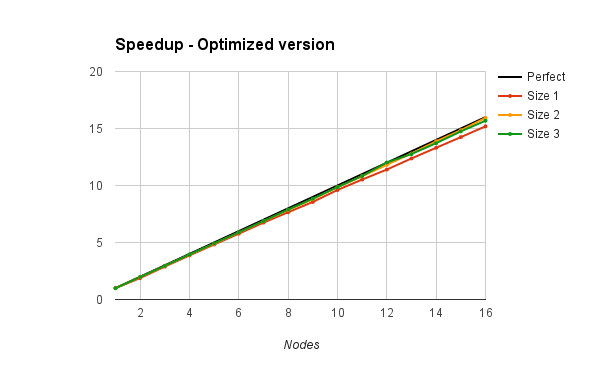
\includegraphics[width=0.8\textwidth]{speedup_improved.png}}
\caption{Speedup - Improved version}
\label{fig:speedupimproved}
\end{figure}

After the implementation of the above improvements, the programs run incredibly faster. The speedup for the three problem sizes can be seen in \autoref{fig:speedupimproved}, while the running times are in \autoref{sec:executiontimes}. \\
It is really unbelievable how much faster the programs are after implementing the improvements, however the programs are still very slow compared to other technologies. Overall, we reached a maximum speedup of 7.6 running on 16 nodes of 8 cores each (256 cores), with respect to the sequential version that uses only 1 core, and this very low performance gain is not acceptable for real application. \\
We can conclude that the Global View approach of Chapel is a very good idea and it simplifies the development process, but there are limitations that cannot be ignored. Until the performance issue won't be solved Chapel cannot be a competitive language, but it is a flexible language that can be used for academic or testing purposes.


\appendix

\section{Bonus work: local view approach}

\section{Execution times} \label{sec:executiontimes}

\begin{table}[H]
\centering
\begin{tabular}{|c|c|c|}
\hline
Size 1 & Size 2 & Size 3 \\
\hline
2.01 & 15.88 & 220.49 \\
\hline
\end{tabular}
\caption{Execution times - Sequential version} \label{tab:sequentialtimes}
\end{table}

\begin{table}[H]
\centering
\begin{tabular}{|c|c|c|}
\hline
Size 1 & Size 2 & Size 3 \\ \hline
0.32 (6.20) & 2.19 (7.26) & 39.71 (5.55) \\ \hline
\end{tabular}
\caption{Execution times - Parallel version} \label{tab:paralleltimes}
\end{table}

\begin{table}[H]
\centering
\begin{tabular}{|l|c|c|c|}
\hline
Nodes & Size 1 & Size 2 & Size 3 \\ \hline
1 & 2.81 (0.71) & 25.31 (0.63) & 380.38 (0.58) \\ \hline
2 & 1.65 (1.22) & 12.50 (1.27) & 218.01 (1.01) \\ \hline
4 & 1.01 (2.00) & 7.27 (2.19) & 110.03 (2.00) \\ \hline
8 & 0.55 (3.63) & 3.69 (4.30) & 51.73 (4.26) \\ \hline
16 & 0.47 (4.28) & 2.22 (7.15) & 29.04 (7.59) \\ \hline
\end{tabular}
\caption{Execution times - Distributed version} \label{tab:distributedtimes}
\end{table}

\end{document}